\documentclass[tikz]{standalone}
\usepackage{pgfplots}
\pgfplotsset{compat=1.15}
\usepackage{mathrsfs}
\usetikzlibrary{arrows,calc}
\usepackage{tkz-euclide}
\pagestyle{empty}

\definecolor{AngleClr}{rgb}{0,0.39215686274509803,0}
\definecolor{ShapeClr}{rgb}{0.6,0.2,0}
\definecolor{SquareClr}{RGB}{250, 248, 217}

\definecolor{ParacircleClr}{RGB}{217,185,7}


\begin{document}

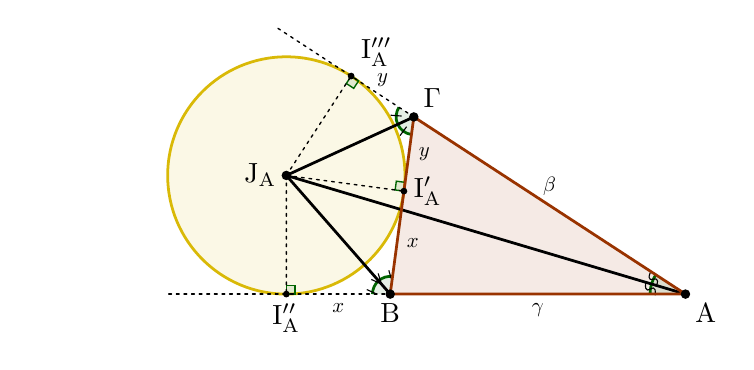
\begin{tikzpicture}[scale=.75]
\tkzSetUpLine[line width=1pt,color=black]
\tkzSetUpPoint[fill=black]

\tkzDefPoints{0/0/B,0.4/3/A,5/0/C}

\tkzDefPointOnLine[pos=-0.2](A,C) \tkzGetPoint{C'}
\tkzDefPointOnLine[pos=-0.2](A,B) \tkzGetPoint{B'}

\tkzDefLine[bisector out](C,A,B) \tkzGetPoint{x}
\tkzInterLL(A,x)(B,C) \tkzGetPoint{D}

\tkzDefPointOnLine[pos=1.2](D,A)\tkzGetPoint{E}

\tkzDefTriangleCenter[ex](B,C,A) \tkzGetPoint{IC}

\tkzDefPointBy[projection=onto B--C](IC)\tkzGetPoint{H}
\tkzDefPointBy[projection=onto A--C](IC)\tkzGetPoint{H2}
\tkzDefPointBy[projection=onto A--B](IC)\tkzGetPoint{H3}

\tkzFillPolygon[fill=ShapeClr,fill opacity=0.1](A,B,C)

\tkzFillCircle[color=ParacircleClr, fill opacity=0.1](IC,H)
\tkzDrawCircle[color=ParacircleClr,line width=1pt](IC,H)

\tkzFillAngle[fill=AngleClr,size=.3,fill opacity=0.1](D,A,B)
\tkzMarkAngle[line width=1pt,size=.3,color=AngleClr,mark=|,mksize=2](D,A,B)

\tkzFillAngle[fill=AngleClr,size=.3,fill opacity=0.1](C',A,D)
\tkzMarkAngle[line width=1pt,size=.3,color=AngleClr,mark=|,mksize=2](C',A,D)

\tkzFillAngle[fill=AngleClr,size=.3,fill opacity=0.1](A,B,IC)
\tkzMarkAngle[line width=1pt,size=.3,color=AngleClr,mark=||,mksize=2](A,B,IC)

\tkzFillAngle[fill=AngleClr,size=.3,fill opacity=0.1](IC,B,H)
\tkzMarkAngle[line width=1pt,size=.3,color=AngleClr,mark=||,mksize=2](IC,B,H)

\tkzFillAngle[fill=AngleClr,size=.6,fill opacity=0.1](A,C,IC)
\tkzMarkAngle[line width=1pt,size=.6,color=AngleClr,mark=s,mksize=2](A,C,IC)

\tkzFillAngle[fill=AngleClr,size=.6,fill opacity=0.1](IC,C,B)
\tkzMarkAngle[line width=1pt,size=.6,color=AngleClr,mark=s,mksize=2](IC,C,B)

\tkzMarkRightAngles[line width=0.5pt, size=.15,color=AngleClr,fill=AngleClr,fill opacity=0.1](IC,H,B IC,H2,A IC,H3,A)

\tkzDrawSegment[line width=0.5pt,color=black,dashed,dash pattern=on 1pt off 1.75pt,add=0.75 and 0](B,C)
\tkzDrawSegment[line width=0.5pt,color=black,dashed,dash pattern=on 1pt off 1.75pt,add=.5 and 0](A,C)

\tkzDrawSegments[line width=0.5pt,color=black,dashed,dash pattern=on 1pt off 1.75pt](IC,H IC,H2 IC,H3)
\tkzDrawSegments[line width=1pt](A,IC B,IC C,IC)

\tkzDrawPolygon[color=ShapeClr](A,B,C)

\tkzDrawPoints[size=3](A,B,C,IC)
\tkzDrawPoints[size=2](H,H2,H3)

\tkzLabelPoint[above right](A){$\rm \Gamma$}
\tkzLabelPoint[below](B){$\rm B$}
\tkzLabelPoint[below right](C){$\rm A$}
\tkzLabelPoint[left](IC){$\rm J_A$}

\tkzLabelPoint[right](H3){$\rm I_A'$}
\tkzLabelPoint[below](H){$\rm I_A''$}
\tkzLabelPoint[above right](H2){$\rm I_A'''$}

\tkzLabelSegment[below](B,H){\scalebox{0.75}{$x$}}
\tkzLabelSegment[right](B,H3){\scalebox{0.75}{$x$}}

\tkzLabelSegment[right](A,H3){\scalebox{0.75}{$y$}}
\tkzLabelSegment[above](A,H2){\scalebox{0.75}{$y$}}
\tkzLabelSegment[below](B,C){\scalebox{0.75}{$\gamma$}}
\tkzLabelSegment[above](C,A){\scalebox{0.75}{$\beta$}}

\end{tikzpicture}
\end{document}
